\documentclass[12pt]{article}
\usepackage{amssymb,amsmath,natbib,graphicx,amsthm,
  setspace,sectsty,anysize,dsfont,enumerate}

\usepackage{times}

\usepackage[svgnames]{xcolor}

\usepackage{lscape,arydshln,relsize,rotating}
\usepackage[small]{caption}
\usepackage{algorithm}

\newtheorem{prop}{\sc Proposition}[section]
\renewcommand{\qedsymbol}{}

\marginsize{1.1in}{.9in}{.3in}{1.4in}

\newcommand{\nb}{\color{blue}}
\newcommand{\dbl}{\setstretch{1.5}}
\newcommand{\sgl}{\setstretch{1.1}}

\newcommand{\bs}[1]{\boldsymbol{#1}}
\newcommand{\mc}[1]{\mathcal{#1}}
\newcommand{\mr}[1]{\mathrm{#1}}
\newcommand{\bm}[1]{\mathbf{#1}}
\newcommand{\ds}[1]{\mathds{#1}}
\newcommand{\indep}{\perp\!\!\!\perp}
\DeclareMathOperator*{\argmin}{argmin}
\newcommand{\norm}[1]{|\!|#1|\!|_{1}}
\newcommand{\cd}[1]{{\tt#1}}
\newcommand{\e}[1]{{\footnotesize$\times10$}{$^{#1}$}}

\sectionfont{\noindent\normalfont\large\bf}
\subsectionfont{\noindent\normalfont\normalsize\bf}
\subsubsectionfont{\noindent\normalfont\it}

\usepackage[bottom,hang,flushmargin]{footmisc}

\pdfminorversion=4
\begin{document}

\sgl 

\pagestyle{empty}

~
\vskip 3cm

\noindent {\huge \bf Distributed Multinomial Regression} 

\vskip 1cm

\noindent{\Large Matt Taddy}

{\large
\vskip .5cm \noindent
{The  University of Chicago Booth School of Business}\\
{\tt faculty.chicagobooth.edu/matt.taddy}}



\vskip 2cm

{\noindent This article introduces a model-based approach to distributed
computing for multinomial logistic regression. We treat
counts for each response category as independent Poisson regressions
via plug-in estimates for fixed effects shared across categories.  The work is
driven by estimation of the high-dimensional-response multinomial models that
arise in analysis of a large number of random counts. Our archetypal
applications are in text analysis, where large sets of documents are tokenized
and the token counts are modeled as arising from a  multinomial dependent upon
document attributes. We estimate such models for a publicly available dataset
of business reviews from the Yelp website, with review text regressed onto a
large set of explanatory variables (user, business, and rating information).
The fitted models then serve as a basis for exploring the connection between
words and variables of interest (e.g., star rating), for reducing dimension
into supervised factor scores, and for prediction. }
 

\newpage
\dbl

\pagestyle{plain}
\vskip 1cm
\section{Introduction}
\label{intro}


The idea is motivated by applications that involve very large response
dimension $D$,  as in multinomial analysis of text counts or other large
categorical datasets (e.g. website visits or consumer purchases).  In
particular, we'll apply the technique to the multinomial inverse regression
(MNIR) of \citet{taddy_multinomial_2013}.  In the original MNIR paper, the
covariate dimension $p$ was small and computation was made extremely fast by
collapsing response counts across level combinations of these  covariates.
DMR extends MNIR to high-dimensional covariate sets where such collapsing is
infeasible.  Beyond MNIR, other authors working in web and text analysis who
previously favored multinomial models -- say, for latent factorization -- are
now using independent Poissons to scale for massive data; see
\citet{gopalan_scalable_2013} as an example.  From the perspective of this
paper, such Poisson modeling strategies can be cast as Big data versions of
their more common multinomial analogues.

These big-$D$ applications have the characteristic that $m_i$ is
random, and usually pretty big.  For example, text mining $m_i$ is the total
word count in document $i$, and web analysis $m_i$ would be the total count of
sites visited by a browser.  A Poisson model for $m_i$ -- the extra assumption
made when moving from a multinomial to independent Poissons -- is not far
fetched, especially if $\bm{v}_i$ includes a large number of covariates and
fixed effects.  However, we also find that DMR does very well for the more
common polychotomous regression setting, where $m_i=1$ always.   In our
polychotomous examples, DMR with lasso penalization and under variety of
selection rules performs at least as well in out-of-sample prediction as a
cross validated lasso on the corresponding multinomial logistic regression
model.  DMR thus provides an every-day speedup in
multinomial regression: even with small-$D$ response
categories, you'll be able to fit the model almost $D$ times faster in
distribution (in simple shared-memory parallelization we observe speedups that
are close to linear in $D$, depending upon machine architecture).

The body of this article starts in Section \ref{MU} with justification of our
plug-in estimator $\hat \mu_i = \log m_i$.  We then review in Section \ref{GL}
penalized estimation and our use of the gamma lasso regularization path
algorithm.  This is followed in \ref{IC} with discussion of coefficient
selection along these regularization paths.  This can either occur on the
basis of the independent Poisson likelihoods, or back on the grouped
multinomial likelihood.  We then break from methodology in Section \ref{M1}
for two simple polychotomous regression examples -- the small forensic glass
data from \cd{R} and a large panel of American light beer purchases.

The second part of the paper begins in Section \ref{MNIR} with an overview of
the MNIR framework of \cite{taddy_multinomial_2013}.  This includes an updated
discussion of the opportunities opened if we allow for larger $D$ than was
considered in the original paper.  Section \ref{MR} provides a MapReduce
algorithm for distributed MNIR in analysis of Big unstructured
datasets.   Finally, we present in Sections \ref{YELP} and \ref{INFER} 
a two-part case study of publicly available Yelp online-review data.   Section
\ref{YELP} considers prediction of review popularity (as scored by other Yelp
users) from text and other attributes.  Section \ref{INFER} describes
inference about the effect of user characteristics while conditioning on
confounding information via text (and makes use of an additional scaling tool:
the weighted least-squares approximation in Appendix \ref{WLS}). We've found
that inference problems of this type are a key application area for MNIR.
Section \ref{END} closes with a quick discussion.

\section{Estimating baseline intensity}
\label{MU}

The likelihood for count data from a set of $D$ independent Poisson trials
factorizes as the product of a multinomial distribution for the individual
counts conditional on the sum total across all trials and a Poisson
distribution on this total.  Say $\bm{c}_i$ is a vector of counts in $D$
categories, summing to $m_i = \sum_j c_{ij}$, and that each $c_{ij}$ has
been drawn independently $\mr{Po}\left(\lambda_{ij}\right)$ -- Poisson with
intensity (i.e., mean) $\lambda_{ij}$. Then the multinomial is `embedded' in
the Poisson: \begin{equation}\label{embed} \mr{p}(\bm{c}_{i}) = \prod_j
\mr{Po}\left(c_{ij};~\lambda_{ij}\right) =
\mr{MN}\left(\bm{c}_i;~\bs{\lambda}_{i}/\Lambda_i,
~m_i\right)\mr{Po}\left(m_i;~\Lambda_i\right), \end{equation} where $\Lambda_i
= \sum_j \lambda_{ij}$ and the multinomial denoted here has probabilities
$\lambda_{ij}/\Lambda_i$ and size $m_i$.

This well known connection has long been used by statisticians to justify
ignoring whether sampling was conditional on margin totals in analysis of
contingency tables. \cite{birch_maximum_1963} showed that the maximum
likelihood estimate (MLE) of $\bs{\lambda}_i$ is unchanged under a variety of
sampling models for 3-way tables {\it under the constraint} that $\Lambda_{i}
= m_i$. This is satisfied at the MLE for a saturated model, with as many
parameters as cells in the table. \cite{palmgren_fisher_1981} extended the
Birch work to log-linear regression models, with $\lambda_{ij} = \exp[\alpha_j
+ \mu_i + \bs{\varphi}_j'\bm{v}_i]$, where $\bm{v}_i$ is a $p$-vector of
covariates, for observations $i=1\ldots n$. The Fisher information on
$\bs{\Phi} = [\bs{\varphi}_1 \cdots \bs{\varphi}_d]'$ is the same regardless
of whether or not you've conditioned on $m_i$ (i.e., in either multinomial
logistic regression or Poisson log regression) so long as $\mu_i$ in the
Poisson model is estimated at its conditional MLE, $\hat \mu_i =
\log\left(m_i/\sum_j e^{\alpha_j + \bs{\varphi}_j\bm{v}_i}\right)$.

Traditionally, this connection is invoked when applying multinomial logistic
regression: totals $m_i$ are then ancillary and the $\mu_i$ drop out of the
likelihood.  This paper takes the opposite view: if we are willing to fix
estimates $\hat\mu_i$ -- potentially not at their MLE -- then the factorized
Poisson likelihood can be analyzed independently across response categories.
Specifically, Section \ref{MU} argues for $\hat\mu_i = \log m_i$ as a plug-in
estimator that minimizes the bias from using Poisson likelihoods in place of a
multinomial for log linear regression. We label this strategy, including
penalized estimation and variable selection within each Poisson, distributed
multinomial regression (DMR).  It is available in the \cd{distrom} package for
\cd{R}.
Consider multinomial logistic regression with linear equations $\eta_{ij} =
\alpha_{j} + \bm{v}_i'\bs{\varphi}_j$ for each observation $i$ and response
category $j$.  The negative log likelihood is proportional to 
\begin{equation}
\label{mnl} \sum_{i=1}^n\left[ m_i\log\left(\sum_{j=1}^D e^{\eta_{ij}}\right)
- \bm{c}_{i}'\bs{\eta}_{i} \right]. 
\end{equation} 
It is easy to verify that adding observation fixed effects $\mu_i$ to each
$\eta_{ij}$ in (\ref{mnl}) leaves the likelihood unchanged.  In contrast, the
corresponding Poisson model, unconditional on $m_i$, has negative log
likelihood proportional to 
\begin{equation} \label{pol}
\sum_{j=1}^D\sum_{i=1}^n\left[ e^{\mu_i + \eta_{ij}} - c_{ij}(\mu_i +
\eta_{ij}) \right] 
\end{equation} 
with gradient on each $\mu_i$ of $g(\mu_i) =
e^{\mu_i}\sum_j e^{\eta_{ij}} - m_i$, and  is clearly sensitive to these
observation `baseline intensities'.  As mentioned above, solution for the
parameters of $\eta_{ij}$ is unchanged between (\ref{mnl}) and (\ref{pol}) if
each $\mu_i$ is set to its conditional MLE at $\log m_i - \log \left[\sum_j
e^{\eta_{ij}}\right]$.

Calculating conditional MLE for baseline intensities $\mu_i$ requires
communication across category dimensions `$j$'. Since distributed computation
precludes such communication, we'll instead use  $\hat \mu_i = \log m_i$ as a
simple plug-in estimator. Conceptually, we justify this choice being also the
conditional Poisson MLE -- the value that would lead  Poisson estimates for
$\eta_{ij}$ to be unchanged from those based on the  joint multinomial
likelihood  -- in a few example models.

From (\ref{pol}), the gradient on $\mu_i$ at this plug-in is $g(\hat \mu_i) =
m_i \left(\sum_i e^{\eta_{ij}}-1\right)$.  Consider a saturated model where
each $\eta_{ij}$ is free.  The Poisson MLE for $\eta_{ij}$ will be $\hat
\eta_{ij} = \log(c_{ij}) - \hat \mu_i = \log(c_{ij}/m_i)$, which gives $g(\hat
\mu_i) = 0$ and this value also minimizes the multinomial likelihood in (\ref{mnl}).   At
the other extreme, consider an intercept-only model with $\eta_{ij} =
\alpha_j$.  The Poisson MLE is $\hat\alpha_j = \log \sum_i c_{ij} - \log
\sum_i e^{\hat\mu_i} = \log\left( \sum_i c_{ij}/M \right)$ where $M = \sum_i
m_i$.  The gradient is $g(\hat \mu_i) = m_i(\sum_j \sum_i c_{ij}/M -1) =
0$ so that we are again at the conditional MLE. Finally, consider a single
binary covariate such that $\eta_{ij} = \alpha_j + x_i \varphi_j$, $x_i \in
\{0,1\}$.  Write $C_{xj} = \sum_{i: x_i=x} c_{ij}$ and  $M_{x} = \sum_{i:
x_i=x} m_i = \sum_j C_{xj}$.  Then the Poisson MLE are $\hat\alpha_j =
\log(C_{0j}/M_0)$ and $\hat\varphi_j = \log(C_{1j}/M_1) - \log(C_{0j}/M_0)$,
so that we retain $g(\hat \mu_i) = m_i\left(\sum_j C_{x_ij}/M_{x_i} -1 \right)
=0$.

These examples do not form a general result (things are more complicated with multiple correlated covariates, and especially under regularization), but they illustrate analytically
why we might expect the performance we've seen empirically: estimates based upon $\hat \mu_i = \log m_i$ do not
suffer in out-of-sample validation. The resulting benefit is huge, as using a
plug-in allows estimation of the Poisson regression equations to proceed in
complete isolation from each other.

\section{Gamma lasso regularization paths}
\label{GL}

Given baseline intensities fixed as $\hat \mu_i = \log m_i$, each of our $D$ separate Poisson
regressions has negative log likelihood proportional to
\begin{equation}\label{obj}
l(\alpha_j, \bs{\varphi}_j) = \sum_{i=1}^n \left[ m_i 
e^{\alpha_j + \bm{v}_i'\bs{\varphi_j}} - c_{ij}(\alpha_j + \bm{v}_i'\bs{\varphi_j})\right].
\end{equation}
This section will describe estimation via regularized minimization of
these objectives. We drop the $j$ response-category subscript for
simplicity.

In high-dimensional analysis, likelihood maximization has been replaced by
penalized likelihood maximization as the estimation tool-of-choice.  Systems
like (\ref{obj}) imply the penalized objective $l(\alpha,\bs{\varphi}) +
n\lambda \sum_k c(\varphi_k)$, where $c$ is some positive cost function and
$\lambda >0$ is a penalty weight.  Such `regularization' has a long history in
engineering (e.g., from Tikhonov): you back away from optimality in exchange
for robustness.  A very common form in statistics is the lasso
\citep{tibshirani_regression_1996}, with $c(\varphi_k) = |\varphi_k|$ an $L_1$
cost function.  The lasso (and other costs with a spike at zero) yield
variable selection: some coefficient estimates will be set to exactly zero.

As the optimal value of $\lambda$ is unknown and must be selected (see Section
\ref{IC} below), efficient implementations of penalized estimation use path
algorithms.  In a `regularization path', one starts at $\lambda_1$ large
enough such that the solution has $\hat\varphi_j=0$ for all $j$.  The penalty
weight is then incrementally decreased and coefficients are updated
accordingly. Since the estimates corresponding to $\lambda_t$ tend to be good
starts for estimation at $\lambda_{t+1}$, such routines are extremely fast
(and a path along, say, 100 $\lambda_t$ values can take less time then solving
for the MLE once).

We will adopt the gamma lasso (GL) approach of
\citet{taddy_gamma_2013}.  That article outlines a simple path
algorithm for $L_1$ penalization with  variable-specific weights $\lambda_t
\omega^t_{k}$.  The GL is `adaptive' in that the  weights at segment
$t+1$ depend on coefficient estimates from time $t$ ($\hat \varphi^t_k$)
through the equation $\omega^{t+1}_k  = \left(1 + \gamma
|\hat\varphi^t_k|\right)^{-1}$ where $\gamma \geq 0$.  This includes the
 lasso if $\gamma=0$.  For $\gamma>0$ it provides fast
`concave' penalization, where  the amount of extra cost applied to
$\hat \varphi$ is {\it decreasing} with the absolute value of this estimate.
Concave penalization implies that strong signals (large $|\hat
\varphi|$) are estimated with nearly zero shrinkage. This is appealing in
analysis of massive datasets, as it allows such signals to include the
effect of any collinear variables and tends to yield sparser $\bs{\hat
\varphi}$ (which is useful in reducing both storage and computation).

Even thought GL paths have this nice feature of diminishing bias, each segment
on the path requires only a simple $L_1$ minimization.  These are solved via
coordinate descent within a Poisson-specific version of iteratively re-weighted least squares (IRLS): the
algorithm in \citet[Section 6]{taddy_gamma_2013} with each iteration's
`observation weights' $\lambda_i$ and `weighted LS response' $\log\lambda_i +
y_i/\lambda_i - 1$.  Here, $\lambda_i = m_ie^{\hat\eta_i}$ is the fitted
intensity at current estimates (recall we're suppressing the $j$  subscript).
A full overview of GL estimation is in the original paper, along with a
general review of concave penalization.  A central theme of the article is
that  one needs to understand the properties of the entire path in order to
pick a single point estimate, $\bs{\varphi}^t$.


\subsection{Selection via Information Criteria}
\label{IC}

Penalized path estimation is a tool for enumerating a set of candidate models:
all those along the grid $\lambda_1 \ldots \lambda_T$.  Think of the weights
$\lambda_t$ as a sort of {\it squelch} that determines what you measure as
signal and what you discard as noise.  The framework is incomplete
without  a way to choose amongst possible $\lambda_t$ values.  This is  a
problem of model selection, and we will address the issue through use of
information criteria \citep[IC; e.g.,][]{efron_estimation_2004}.  

We choose amongst  candidate
parameter estimates $\{\bs{\hat\Theta}_1 \ldots \bs{\hat\Theta}_1 \}$ to
minimize \begin{equation}\label{cp} \text{IC}(k) = 2l(\bs{\hat\Theta}_t ) +
k\times df \end{equation} where $2l$ is fitted deviance,   $k$ is a complexity
penalty and $df$ is the number of degrees of freedom in minimization of $l$,
the negative log likelihood.   For the standard lasso, $df$ is simply the
number of nonzero parameters \citep{zou_degrees_2007}, while
\cite{taddy_gamma_2013} provides a heuristic for calculating $df$ under
different levels of concavity in the gamma lasso.

There are two possible ways that IC can be applied in DMR.  The first, perhaps more obvious, option has $\bs{\Theta}$ the full set of multinomial parameters, $[\bs{\alpha},\bs{\Phi}]$, and $2l$ is multinomial deviance.  This scheme leads to a number of computational bottlenecks: since $\lambda_t$ selection is shared across response categories, each 
 Poisson regression regularization path needs to run on the same grid of penalty weights.  Moreover, the full coefficient paths need to be passed back to a central machine for evaluation of multinomial deviance at each path segment (which can itself be expensive, due to the normalization required in calculating a multinomial likelihood).  

As an alternative, we advocate independent {\it ungrouped} IC selection for each individual Poisson regression: there are $D$ unique $\bs{\Theta} = [\alpha_j,\bs{\varphi}_j]$ and $l$ is 
the corresponding Poisson deviance.  We do not include $\hat \mu_i = \log m_i$ in the degrees of freedom accounting, such that $df_j$ based on only $[\alpha_j,\bs{\varphi}_j]$.
In this set-up each Poisson regression has its own
regularization path and selected coefficients correspond to a unique penalty weight $\lambda^t_j$.  This speeds up computation by allowing calculation of initial $\lambda^1_j$ to occur in parallel, by limiting communication to only the coefficient estimates at selected $\lambda^t_j$ (instead of the entire paths), and by eliminating the need for any full multinomial likelihood evaluation.  Moreover we find -- despite what we may have hypothesized about the benefits of grouped selection -- that the independent Poisson model IC selection performs at least as well as grouped multinomial selection in OOS validation.  

The two most common IC rules are the AIC, with $k=2$, and BIC, with
$k=\log(n)$. Our experience is that with large $n$ the BIC selects overly
simple models, while for more covariates than observations the AIC overfits.
The two options act as informal bounds on model complexity.
In the examples here (which always have larger $n$ than number of
covariates), the AIC is the best performer by a large margin in both grouped and independent selection.  

Note that IC model selection is somewhat nonstandard  -- cross validation
(CV), the procedure of looping over out-of-sample (OOS) prediction on 
left-out folds (subsets) of your data, is probably more common.  We focus on IC here, and use CV only for validation of our various IC techniques, because the intent of the work is to offer massive scalability. Monte Carlo routines require significant extra time and communication overhead (plus thread-safe random number generation).  However, there is  nothing inherently wrong with CV selection in DMR; we hypothesize that CV rules applied to each independent Poisson regression will do very well.

\section{Polychotomous regression examples}
\label{M1}

Before moving to big-$D$, MNIR, and our Yelp case study, we look at the
(surprisingly strong) performance of DMR in simple $m_i=1$ polychotomous
regression.

\subsection{Glass shards}
\label{FGL}


\begin{figure}
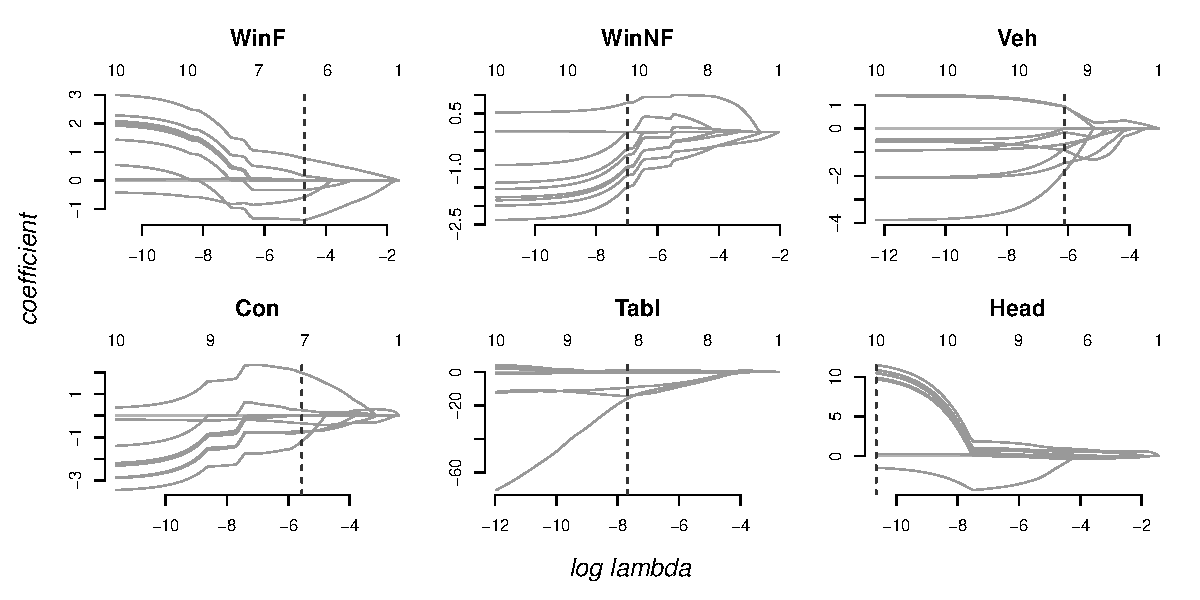
\includegraphics[width=6.25in]{../graphs/fgl_coef}
\caption{\label{fgl_coef} {\it Forensic Glass}. Regularization paths for each glass-type response category.  AIC and BIC selections are marked with dashed vertical lines (orange and green respectively; they overlap for \cd{Tabl}).}
\vskip 1cm
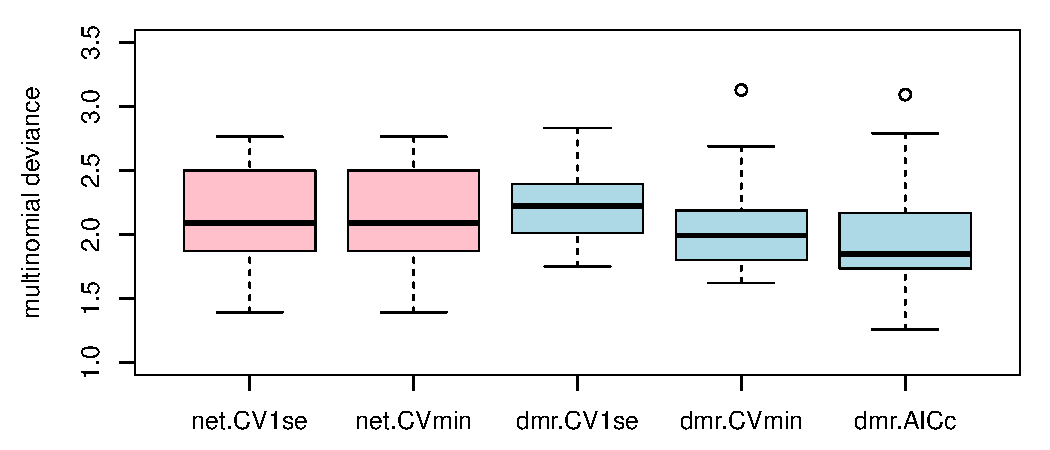
\includegraphics[width=6.25in]{../graphs/fgl_cv}
\caption{\label{fgl_cv}  {\it Forensic Glass}. OOS deviance for \cd{dmr} and \cd{glment} in 20 fold CV.  Dots are mean and segments show $\pm$ 1se.  The vertical dashed lines mark CV and IC shared $\lambda_t$ selections, with black for CV (min and 1se), green BIC and orange AIC. Horizontal lines are mean OOS deviance for response-specific IC selections. The top axis is the mean number of nonzero coefficients across response categories.}
\end{figure}

Our first illustration uses the small `forensic glass' dataset from
\citet{venables_modern_2002}, available in the \cd{MASS} library for \cd{R}
under the name \cd{fgl}.  The data are 214 observations on fragments of glass
collected in forensic work. The response of interest is glass type: window
float glass (\cd{WinF}), window non-float glass (\cd{WinNF}), vehicle window
glass (\cd{Veh}), containers (\cd{Con}), tableware (\cd{Tabl}) and vehicle
headlamps (\cd{Head}).  Covariates for each shard are their refractive index
and \%-by-weight composition amongst 8 oxides.

The response here is a single category, such that $m_i = 1$ and $\hat\mu_i=0$
for all $i$.  This clearly violates the assumption of Poisson generation:
$m_i=1$ is not random.  However, \cd{dmr} still works:  multinomial models
obtained from the fitted Poisson model regularization paths, either using IC
or CV selection, perform as well as CV selected models from a lasso path for
multinomial logistic regression (as implemented in the \cd{glmnet} package for
\cd{R}).  Maximum OOS $R^2$, calculated for multinomial deviance, is about
33\% for both.

Poisson lasso (GL with $\gamma=0$) regularization paths for each glass type
are shown in Figure \ref{fgl_coef}, with the selected coefficients marked for
AIC and BIC applied independently to each Poisson model.  Out-of-sample
performance is illustrated in the left panel of Figure \ref{fgl_cv}, and can
be compared against that of \cd{glmnet} in the right panel.  Here, and
throughout this paper, we use the same 20 folds for both DMR and \cd{glmnet}
experiments.  The vertical lines mark shared $\lambda$ values from grouped
model selection, via IC or CV rules, based on multinomial deviance.  In the
left plot, the two horizontal lines mark average multinomial OOS deviance for
independent IC selection of distinct $\lambda$ values for each response
category (based on the Poisson deviances).  All selection criteria return
values with average OOS deviance within one standard error of the minimum
average value.  For each IC, the independent Poisson selections are more
heavily penalized than their group-learned multinomial-based counterparts.  As
we will see again in later examples, independent Poisson-based AIC selection
is the top performer.

\section{MNIR}
\label{MNIR}

The previous section shows DMR as a tool for $D\times$ speedups in
polychotomous regression.  However, the procedure is really motivated by
multinomial applications with large $D$.  Our main application is multinomial
inverse regression \citep[MNIR][]{taddy_multinomial_2013}, a framework for
building supervised reduced dimension representations of high dimensional
count data.  This section outlines MNIR, which will be applied with DMR in our
Yelp case study of Section \ref{YELP}.

Inverse regression (IR) is a general strategy for dimension reduction when
trying to predict $K$ dimensional attributes $\bm{v}_i$ from high dimensional
(say, of length $D \gg K$) covariates $\bm{x}_i$.  IR is a three stage
procedure: first, fit an {\it inverse model} for $\bm{x}_i | \bm{v}_i$;
second, use the inverse model to obtain {\it sufficient reduction} (SR) scores
$\bm{z}_i$ as reduced dimension projections from $\bm{x}_i$; third, fit a low
dimensional {\it forward regression model} for $\bm{v}_i | \bm{z}_i$.   In
this process the inverse distribution takes the form $\bm{x}_i \sim
f(\bs{\Phi}\bm{v}_i)$, where $f$ is some parametric (typically natural
exponential family) distribution that depends upon $\bm{v}_i$ through the
linear operator $\bs{\Phi}$, a $D\times K$ matrix of loadings.  The SR
projection is then the $K$-vector $\bm{z}_i = \bm{x}_i'\bs{\Phi}$. Under
certain conditions, it  holds that $\bm{x}_i \indep \bm{v}_i \mid \bm{z}_i$.
Thus all information in $\bm{x}_i$ relevant to $\bm{v}_i$ is summarized in
$\bm{z}_i$, and to predict $\bm{v}_i$ we need model only the $K$-variate
regression of $\bm{v}_i$ on $\bm{z}_i$. See \citet{cook_fisher_2007} for an
overview.

The reason one would want to use IR is its efficiency.  Say $D$, the dimension
of $\bm{x}_i$, is big relative to $n$ and that estimation of the parameters in
$\bm{v}_i |\bm{x}_i$ has a high sampling variance.  Assuming an inverse model
$f(\bm{x}_i | \bm{v}_i)$ introduces information into the estimation problem (a
less generous term is `bias') by restricting the relationship between
$\bm{x}_i$ and $\bm{v}_i$ to the possibilities parameterized by $f$.  If $f$
is close enough to the truth then this restriction will be useful.  Cook's
paper includes rigorous efficiency results.  We've found it helpful to make
analogy to the simple arguments used in the related setting of generative
classifiers \citep[e.g., as in][for Gaussian
discrimination]{efron_efficiency_1975}: you  assume higher asymptotic error
rates (since $\bm{x}_i$ is a higher dimensional random variable to be modeling
than $\bm{v}_i$) in exchange for getting near to the optimal rate faster
(e.g., through conditional independence assumptions in the inverse/generative
distribution).

\cite{taddy_multinomial_2013} introduced multinomial inverse regression 
as a version of IR for dealing with $\bm{x}_i = \bm{c}_i$, covariates that can
be characterized as high-dimensional count data.  Our primary application is
in text mining, where $\bm{c}_i$ is a vector of word (or token, phrase,
etc) counts and $D=\mr{length}(\bm{c}_i)$ is the size of the vocabulary.  The
model is just logistic regression, with $\eta_{ij} = \alpha_j +
\bm{v}_i'\bs{\varphi}_j$ the linear model parametrization for the $j^{th}$
response category (e.g., word) from the $i^{th}$ observation (e.g., document).
Given $\bs{\hat\Phi} = [\bs{\hat\varphi}_1 \cdots \bs{\hat\varphi}_D]'$
estimated for this logistic regression, MNIR sufficient reduction scores are
$\bm{z}_i = \bm{c}_i'\bs{\hat\Phi}/m_i$ and we have that $\bm{v}_i \indep
\bm{c}_i \mid \bm{z}_i, m_i$. The $1/m_i$ multiplier on here moves projection
from word counts to proportions, as in
\cite{taddy_multinomial_2013}, and sufficiency for $\bm{z}_i$ is dependent
upon $m_i$ because we've conditioned on these totals in the 
multinomial model.  The algorithm is completed with forward prediction for $\bm{v}_i$ given $[\bm{z}_i,m_i]$; Section \ref{YELP} uses both simple linear regression and a random forest algorithm.

Analysis, examples, applications of the MNIR framework are in
\cite{taddy_measuring_2013,taddy_multinomial_2013,taddy_rejoinder:_2013}. 
There are a number of benefits of the approach.  First, the IR efficiency
argument is especially simple: assuming a multinomial distribution
implies that each of the $M = \sum_i m_i$ count elements are independent
observations, such that the sample size for learning $\bs{\Phi}$ is now $M$
rather than $n$.  That is, in text mining, estimation variance decreases with
the number of words rather than the number of documents. Moreover,
as we see below via our use of random forests, working with the lower dimensional $\bm{z}_i$ scores allows us to apply powerful nonlinear and ensemble learners that would be infeasible (and unstable) on the full dimensional $\bm{x}_i$.

Another advantage of MNIR is business oriented: it is a practical way to
organize information.  In Big data environments, the $\bm{v}_i$ typically
contain subsets of attributes that will variously be treated as known or
unknown (i.e., conditioned upon or predicted) in future analyses.  For
example, at a marketing firm $\bm{c}_i$ could be counts for website visits by
a specific computer, while $\bm{v}_i$ contains geographic and demographic
information along with any observed purchasing behavior.
Given a fitted MNIR, the massive set of $\bm{c}_i$ counts can be
made available in compact $\bm{z}_i$ scores after mapping through
$\bs{\Phi}$.  For the analyst to include text data in any modeling related to
$\bm{v}_i$ they then need only grab the relevant dimensions of $\bm{z}_i$.
We'll see this tactic in practice in Section \ref{YELP}:  text
projections on review popularity used first in prediction, and then
augmented with projections onto user characteristics for an inference problem.

The final advantage of MNIR has been computational.
\cite{taddy_multinomial_2013,taddy_measuring_2013} work with very small
attribute sets, where $K<10$ and often $K=1$.  Since sums of multinomials with
equal probabilities are are also multinomial, one can then {\it collapse} the
modeled counts across equal level-sets of the covariates without affecting the
likelihood (continuous covariates can be binned to facilitate collapsing).
For example, if $v_i$ is a univariate binary attribute (e.g., whether a
speaker is Republican in the original MNIR paper) then the logistic multinomial regression
  has only two observations: the combined counts
corresponding to each of $\{i:v_i=0\}$ and $\{i:v_i=1\}$. Since collapsing can
occur independently for each dimensions of $\bm{c}_i$,  MNIR  even
works in settings where the original $n\times D$ count data is too big to
store on a single machine.

However, there are many settings with attributes of  larger dimension, say $K$
on the order of hundreds or thousands, where such collapsing is impossible.In
Section \ref{YELP} we have over 400 variables of meta-data associated with
each restaurant review.  Moreover,  the MNIR model is not very believable if
$K$ is small -- it seems implausible that only a few factors of interest
explain the heterogeneity between individual document word counts. The
arguments in \cite{taddy_multinomial_2013,taddy_rejoinder:_2013} explain how
MNIR can work even if the inverse model is misspecified on an individual level
(but is a good fit to the collapsed data).  However, there are many settings
where this will not hold, and the argument does not apply if you want to
interpret individual parameters. In such applications one needs to
include a big-$K$ set of explanatory attributes, possibly including many fixed
or latent effects.   This requires a new computational framework, and it has
driven development of DMR.  The distribution allows MNIR to work on a
previously impossible scale.

\section{A MapReduce algorithm} 
\label{MR}

We now outline a MapReduce algorithm for analysis of unstructured  data via
distributed MNIR.   MapReduce \citep[MR;][]{dean_mapreduce:_2004} is a  recipe
for analysis of massive datasets, designed to work when the data itself is
distributed: stored in many files on a network of distinct machines.
The most common platform for  MR is Hadoop paired with a distributed file-
system (DFS)  optimized for such operations (e.g., Hadoop DFS or
Amazon's S3 storage).

A MapReduce routine has three main steps: map, sort, and reduce.  The sort  is handled by 
Hadoop, such that the statistician need worry only about map and reduce.  The map operation parses  unstructured data into a special format.  For us, in a text mining example, the mapper program will take a document as input, parse the text into tokens (e.g. words), and output lines of processed token counts: `\cd{token   document|count}'.  The pre-tab item (our \cd{token}) is called a `key'.  Hadoop's sort facility uses these keys to send the output of your mappers to machines for the next step, reducers, ensuring that all instances of the same key (e.g., the same word) are grouped together at a single reducer.  The reducer then executes some operation that is independent-by-key, and the output is written to file (usually one file per reducer).

Distributed MNIR fits nicely in the MR framework.  Our map step tokenizes your unstructured data  and organizes the output by token keys.  Reduce then takes all observations on a single token and runs a Poisson log regression, applying the gamma lasso with IC selection to obtain coefficient estimates.  These are used to build our SR scores, which can be employed in forward regression after the MR routine is done.  This recipe is detailed in Algorithm \ref{mralgo}.

\vskip .2cm
\begin{algorithm}[h!]
\caption{\label{mralgo} Distributed MNIR }
\vskip .25cm
{\bf Map:}  For each document, tokenize and count sums for each token.  Save the total counts $m_i$ along with attribute information $\bm{v}_i$. Output \cd{token   document|count}.

\vskip .25cm
Combine totals $m_i$ and attributes $\bm{v}_i$ into a single table, say \cd{VM}. This info can be generated during map or extracted in earlier steps.  Cache \cd{VM} so it is available to your reducers.

\vskip .25cm
{\bf Reduce:} For each token key `$j$', obtain a regularization path for Poisson regression of counts $c_{ij}$ on attributes $\bm{v}_i$ with $\hat\mu_i = \log m_i$.  Apply AIC to select a segment of coefficients from this path, say $\bs{\hat\varphi}_j$, and output nonzero elements in sparse triplet format: \cd{word|document|count}. 

\vskip .25cm
Each reducer maintains a running total for SR projection, $\bm{z}_i \stackrel{+}{=} \bm{x}_i'\bs{\hat \varphi_j}/m_i$, output as say \cd{Z.r} for the $r^{th}$ reducer.  When all machines are done we aggregate \cd{Z.r} 
to get the complete projections.  

\vskip .25cm
The final output is the $n \times K$ table \cd{Z} (or with $<K$ columns if you don't need all projection dimensions).  The framework is completed in forward regression with \cd{Z} and \cd{VM}. 
\vskip .5cm
\end{algorithm}



We've written this as a single MR algorithm, but other variations may work better for your computing architecture. Our most common implementation uses streaming Hadoop on Amazon Web Services (AWS) to execute the map on a large number of files in AWS S3 cloud storage, but replaces the regression reduce step with a simple write, to solid state storage `midway' at the University of Chicago's Research Computing Center, of token counts tabulated by observation.  For example, given 64 reducer machines on AWS the result is 64 text tables on midway, with lines `\cd{word|doc|count}', each containing {\it all} nonzero counts for a subset of the vocabulary of tokens.  These files are small enough to fit in working memory\footnote{If not, use more reducers or split the files.} and can be analyzed on distinct compute nodes, each employing another layer of parallelization in looping through Poisson regression for each token.  This scheme is able to take advantage of Hadoop for fast tokenization of distributed data, and of
high performance computing architecture (much faster than, say, a virtual AWS instance) for distributed  regression analyses.  This is a model that should work well for the many statisticians who have access to computing grids that are designed for high throughput tasks more traditionally associated with physics or chemistry.


\section{Yelp review popularity prediction}
\label{YELP}

These data were supplied by the review site Yelp for a data mining contest on \cd{kaggle.com}.  Full details are at \cd{www.kaggle.com/c/yelp\!-\!recruiting/data}; we'll consider the business, user, and review datasets.  The reviews, of all sorts of businesses, were recorded on January 19, 2013 for a sample of locations in the southwest US (mostly around Phoenix AZ).  The goal of the competition was to predict the combined number of `funny', `useful', or `cool' (f/u/c) votes that a given review receives from other users.  Such information can be used by yelp to promote f/u/c  reviews before waiting for the users to grade them as such.  
The example is typical of the problems we encounter in data mining, while it has the advantage that it is publicly available and not so large that we cannot -- for comparison -- also analyze and cross validate in-memory using a standard lasso.

After removing reviews by unknown users, the data are $n=$ 215,879 reviews on
11,537 businesses by 43,873 users. Business-specific covariates include review-
count, star-average, and location, which we model through 61 city
fixed effects on top of state effects.  Yelp also records a non-exclusive
taxonomy of business types; we track membership information for each of the
333 categories  containing more than 5 businesses. User covariates are
limited to information about past reviews on Yelp: the user's total review count
(\cd{usr.count}), their average number of stars given (\cd{usr.stars}), and
their previously accumulated count of f/u/c votes (\cd{usr.funny},
\cd{usr.useful}, \cd{usr.cool}; for each observation we subtract that
review's f/u/c votes from these totals). Review text was tokenized into
words (including combinations of punctuation: potential emoticons) separated
by whitespace. After stripping some common suffixes (e.g., `s', `ing', `ly')
and removing a small set of stopwords (e.g., `the', `and', `or'), we counted
frequencies for $D=$ 13,938 words occurring in more than 20 ($< 0.01\%$) of
the reviews (total word count is $M=$ 17,581,214).  In addition to the text,
review data includes the star rating and time ($t$ and $t^2$)
measured in days since posting.  Code for tokenization and data processing
(and for all the estimation in this section) is available at
\cd{github.com/mataddy/yelp}.

 
This yields the following components for our analysis:  an $n \times D$
review-word frequency matrix $\bm{C} $ and $n$-vector of row-totals  $\bm{m}$;
the $n \times 408$ matrix $\bm{U}$ of business, user, and non-text review
covariates; and the $n \times 9$ matrix $\bm{V}$ containing each f/u/c vote
count by type and its interaction with the time variables, $[t,t^2]$.  Columns of both
$\bm{U}$ and $\bm{V}$ are scaled to have a standard deviation of one. The
multinomial inverse regression model is then
\begin{equation}
\bm{c}_i \sim \mr{MN}(\bm{q}_i, m_i),~q_{ij} = e^{\eta_{ij}}/\sum_{l}e^{\eta_{il}},
~\text{where}~\eta_{ij} = \alpha_j + \bs{\varphi}_j^{u}\bm{u}_i + \bs{\varphi}_j^{v}\bm{v}_i.
\end{equation}
Each distributed Poisson likelihood that we fit, using $\hat\mu_i = \log m_i$, has the form,
\begin{equation}
c_{ij} \sim \mr{Po}\left(m_ie^{\eta_{ij}}\right) = 
\mr{Po}\left(m_i\exp[\alpha_j + \bs{\varphi}_j^{u}\bm{u}_i + \bs{\varphi}_j^{v}\bm{v}_i]\right)
\end{equation}
with corresponding negative log likelihood proportional to
\begin{equation}
l_j = \sum_i m_i e^{\eta_{ij}} - c_{ij} \eta_{ij} 
= \sum_i m_i \exp[\alpha_j + \bs{\varphi}_j^{u}\bm{u}_i + \bs{\varphi}_j^{v}\bm{v}_i]
- c_{ij}(\alpha_j + \bs{\varphi}_j^{u}\bm{u}_i + \bs{\varphi}_j^{v}\bm{v}_i).
\end{equation}
Gamma lasso regularization paths of $20$ $\lambda_t$ values are fit
 for each independent Poisson regression.  
We use $\gamma =1$ in the GL algorithm to achieve concave penalization via
path adaptation. Point estimates $\bs{\hat\varphi}_j$
are selected using AIC based on independent
Poisson deviances.  We do not consider grouped multinomial-based selection here because of its computational expense.


Regularization paths for a few of the Poisson models  are shown in Figure
\ref{yelp_ir}.  We see, for example, that at our AIC selection the effect of a
1sd increase in review stars multiplies the expected count (or odds, in the
multinomial model) for token \cd{:-)} by around $\exp 0.35 = 1.4$ and for
token \cd{:-(} by around $\exp -0.4 = 0.7$.  In the estimates of our
regression model for counts of token \cd{sex}, we see that the word is
positively associated with funny votes but negatively associated with useful
votes (1sd extra \cd{funny} increases \cd{sex} by around 60\%, but 1sd extra
\cd{useful} corresponds to a 30\% drop in expected \cd{sex}).

\begin{figure}
\hspace{-.25in}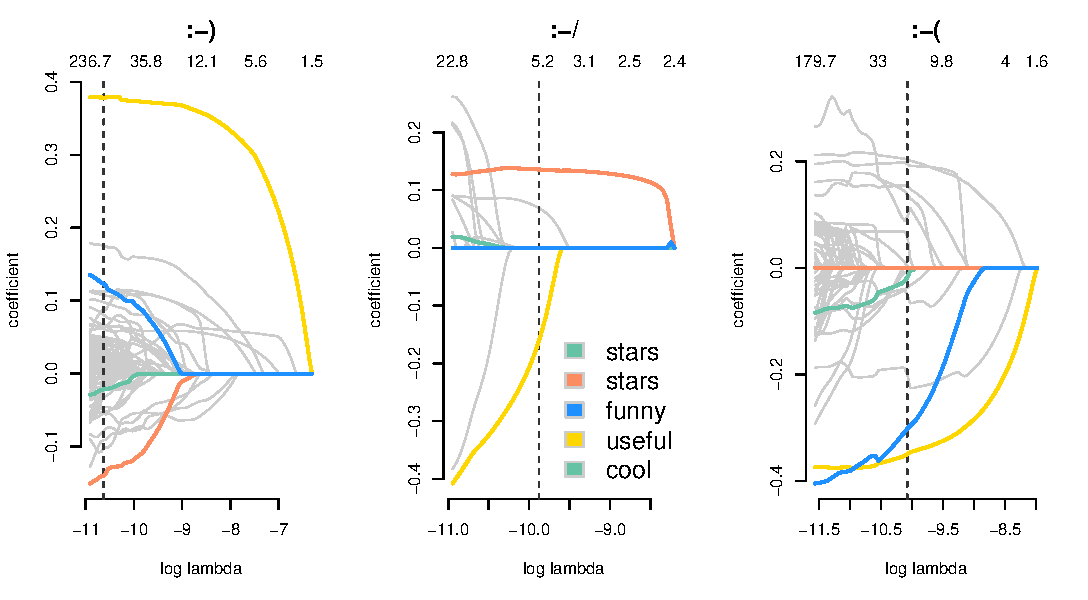
\includegraphics[width=6.75in]{../graphs/yelp_ir_paths}
\caption{\label{yelp_ir} {\it Yelp}.  Inverse regression coefficient
regularization paths for counts of the tokens \cd{:-)}, \cd{:-(}, and \cd{sex}
regressed onto covariates $[\bm{u},\bm{v}]$.  The legend highlights select
covariates, Poisson model degrees of freedom are on the top axis, and our AIC
selected estimates are marked with vertical dashed lines. }
\end{figure}

Turning to forward regression, denote combined f/u/c votes -- the response of
interest -- by the $n$-vector $\bm{y}$. We consider prediction of
$\log(y_i+1)$ using covariates $\bm{u}_i$, review length $m_i$, and the SR
projections $\bm{z}_i^v = (1/m_i)\bm{c}_i'\bs{\Phi}^v$, with $\bs{\Phi}^v =
[\bs{\varphi}^v_1 \cdots \bs{\varphi}^v_9]'$  coefficients for the nine
f/u/c$\times [1,t,t^2]$ variables in $\bm{v}_i$.  Note that we use text SR
factors only for variables derived from $y_i$; projection onto $\bm{u}_i$ is
ignored unless, as in Section \ref{INFER}, we want to reduce bias in estimation of
coefficients on  $\bm{u}_i$. Two algorithms are applied for predicting
$\log(1+\bm{y})$ from $[\bm{U},\bm{Z}^v,\bm{m}]$: ordinary least-squares (OLS), and
a 1024 tree random forest \citep[RF;][]{breiman_random_2001} as implemented in the
\cd{randomForest} package for \cd∫{R}. Results from a 20-fold CV (with each fold left-out for both IR and forward regression)
are shown in Figure \ref{yelp_cv}.  For comparison, we also
show results of straightforward lasso linear regression onto the 13,938 + 1 +
408 =  14,347 column input matrix $[\bm{C}/\bm{m},\bm{m},\bm{V}]$, where
rows of $\bm{C}/\bm{m}$ are word proportions $\bm{c}_i/m_i$.

\begin{figure}
\vskip -.2cm
\hskip .5in 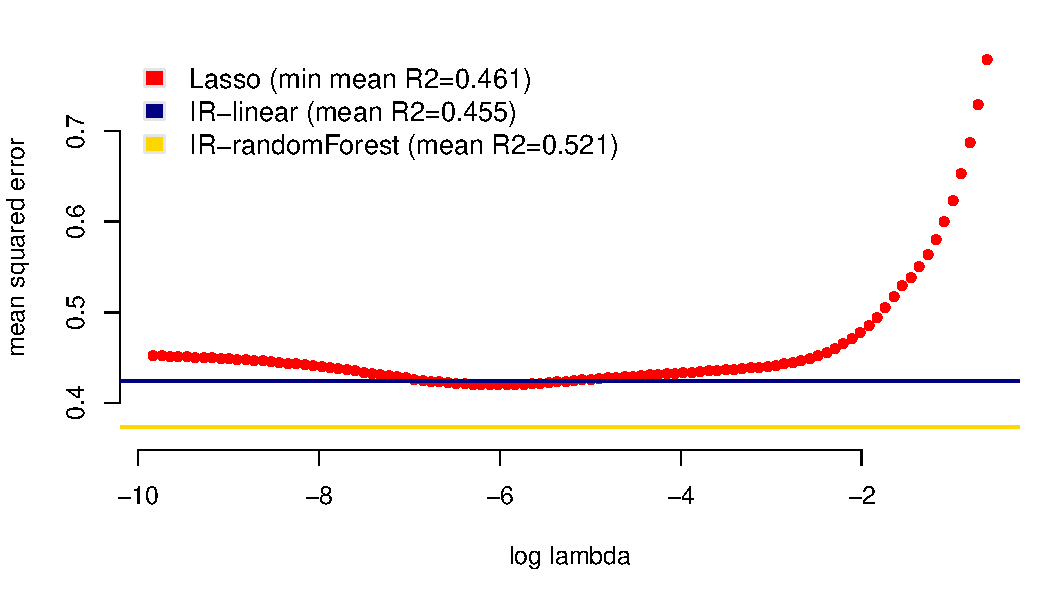
\includegraphics[width=5.2in]{../graphs/yelp_cv}
\vskip -.2cm
\caption{\label{yelp_cv} {\it Yelp}.  20-fold OOS  prediction of $\log(y_i +1)$, where $y_i$ is a reviews combined f/u/c votes.  For both inverse regression
(IR) procedures, penalization was selected inside the experiment via independent Poisson AIC.  The lines and points mark mean OOS MSE, and standard errors are too narrow to see. }
\end{figure}


Figure \ref{yelp_cv} shows that average performance of the IR-linear algorithm
(MNIR + OLS), using AIC model selection for IR coefficients, is no better than
the best straightforward lasso specification (although MNIR is being put to a
tougher test here: selecting penalization {\it within} the CV experiment
instead of finding the fixed penalty that performs best across folds). Such
performance is  typical of what we've observed in Big data application.
\footnote{In the comparisons of \cite{taddy_multinomial_2013}, the IR linear
model consistently outperforms a linear lasso comparator in OOS prediction and
in compute time.  However, the datasets used in that paper are both very
small, with $M\gg n$.  Thus the simple argument in the rejoinder
\cite{taddy_rejoinder:_2013} Proposition 1.1 -- that, for multinomial IR,
estimation variance decreases with $M$ instead of $n$ -- is working heavily in
favor of IR. Examples like the yelp application here are more typical in Big
data: even though $M > n$, the vocabulary size $D$ is smaller than $n$ and
straightforward linear regression is already plenty efficient.}   The
advantage of MNIR with linear forward regression is then computational: it
works in complete distribution  and is thus massively scalable (we see in
Section \ref{INFER} that the multinomial model is also useful for structural
inference).  However the random forest results show another advantage of MNIR:
one can deploy flexible nonlinear machine learning on the low dimensional
space resulting from SR projection. Methods that are too computationally
expensive or unstable on the full covariate set are easy
and fast to run on the reduced dimension subspace; our experience with tree
methods finds much rich interaction structure that can be exploited after MNIR
dimension reduction.

\section{Inference: estimating the user effect}
\label{INFER}

Machine learning feats are nice -- e.g., OOS $R^2$ greater than 50\% on the
log number of f/u/c votes -- but for staff at Yelp it is likely more important
to understand the sources of variation.  When a new review is written for a
specific business, Yelp can only promote (or not promote) it relative to
reviews on the same page.  The question is not `how popular will this review
be?', but rather `should we promote this review over others for this
business?'  One way to answer looks at the users: are there certain people who
write better reviews?  This creates an inference problem -- we want to
estimate the real effect of user characteristics. This section first describes
effect estimation under the setup of Section \ref{YELP}, before investigating how
inference can be improved by conditioning on additional SR projections.

\begin{figure}[t]
\vskip -.5cm
\hskip .5in
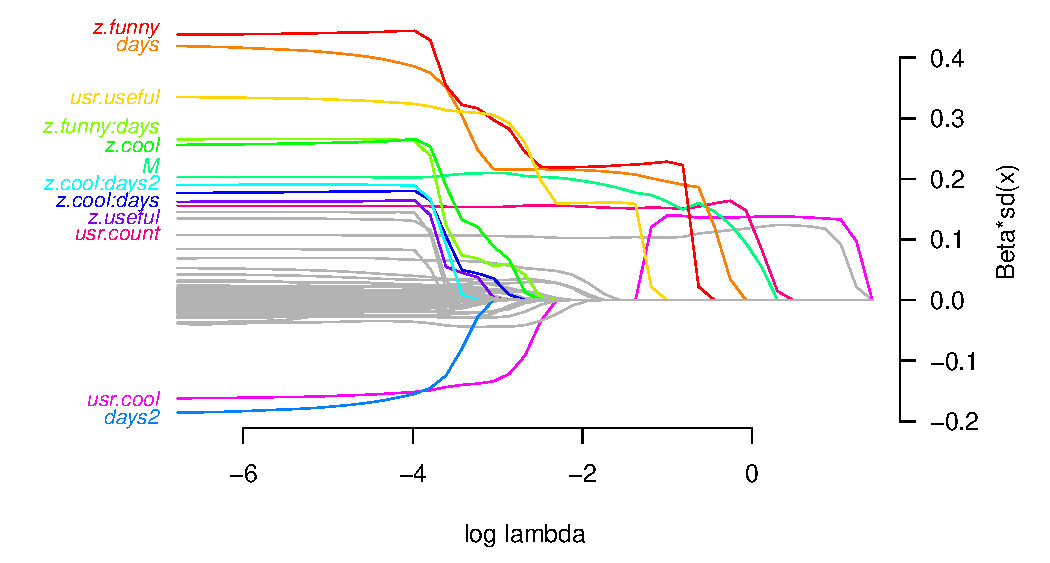
\includegraphics[width=5.2in]{../graphs/yelp_fwd_paths}
\caption{\label{yelpfwd} {\it Yelp.}  Forward Poisson log regression of combined f/u/c vote counts onto review attributes $\bm{u}_i$ and text-vote projections $\bm{z}^v_i$.  These are gamma lasso paths with high concavity ($\gamma=10$). }
\end{figure}

 Figure \ref{yelpfwd} shows regularization paths for
Poisson regression (full generalized linear model, not a linear model for
log $y$) of  counts $y_i$ on   $\bm{u}_i$ and
$\bm{z}^v_i$.  This is a gamma lasso fit with $\gamma =10$, for a very concave
penalty (little bias), such that estimates at the end of the path
are near the corresponding MLE.  As in any multivariate regression, these coefficients
represent {\it partial effects} --  change due to
 individual covariates {\it after} controlling for the effect of all other
inputs.  Consider the coefficient on \cd{usr.cool}, a user's historical
count of `cool' votes.  This has a negative partial effect (around -0.17 at
minimum penalty), despite having a big positive marginal effect (if you follow
the path, you'll see that \cd{usr.cool} is actually the first covariate to
enter the model).  Thus after you account for the quality
predictable by funny or useful votes (particularly useful, which is about
twice as common as the others), extra cool votes indicate someone less likely
to write popular reviews.  This situation occurs because the individual
category votes are highly collinear, with correlations between each other of
0.7 to 0.9.

\subsection{Improved treatment effect estimation}

Inference about regression parameters is notoriously difficult in the presence of high dimensional collinear controls.  Likelihood maximization for the full 14,347
variable regression in our Yelp example, of vote count on all attributes and all text counts,  would be very expensive and implies only around 15 observations per covariate.  
In larger problems, $n$ and $\mr{dim}(\bm{x}_i)$ may be so large that such a regression is computationally impossible.
Unfortunately, the tools that we would usually employ for variable selection (such as a straightforward lasso) will yield biased effect estimates.  To see this, consider
the regression 
\begin{equation}\label{teffects}
\ds{E}[\log y_i] = \beta_0 + d_i\theta  + \bm{x}_i'\bs{\beta}
\end{equation}
where $d_i$ is our `treatment' (e.g., user characteristic), $\theta$ is
the effect of interest, and $\bm{x}_i$ is a large vector of control
variables (e.g., all other review attributes and the token counts).   There
will surely be elements of $\bm{x}_i$ that are correlated with $d_i$. If
we estimate $\bs{\beta}$ under lasso penalization, 
then $\hat\beta_j \neq 0$ only if there is 
residual effect of $x_{ij}$ beyond that which can be regressed on $d_i$.  The
 effect for these treatment-collinear variables will be conflated
into $\hat\theta$, leading it to be mis-estimated simply because $d_i$ is correlated with many
variables who's effect has been underestimated.  The efficiency of the lasso
for prediction is now working against us in inference.

In contrast, because the text covariates, $\bm{c}_i$, enter only through the 9
dimensional SR projection $\bm{z}^v_i$, we are able to use likelihood maximization
 to estimate the partial effects of Figure \ref{yelpfwd}.
We can improve these estimates still by adding the SR
projections $z^u_{ik}$ corresponding to the treatments of interest.    To see why, look
again to the treatment effects regression in (\ref{teffects}): 
unbiased estimation of $\theta$ needs $\bs{\hat\beta}$ to account both for
predictability of $\log y_i$ from $\bm{x}_i$ and of $d_i$ from $\bm{x}_i$.  To
put it another way, an ideal version of (\ref{teffects}) would have $\ds{E}[\log y_i] = \beta_0 + d_i\theta  + \beta_y \ds{E}[\log y_i
| \bm{x}_i] + \beta_d \ds{E}[d_i | \bm{x}_i]$.  Without the $\beta_d \ds{E}[d_i | \bm{x}_i]$ 
term, estimated $\hat\theta$ will be confounded with any effects from
$x_{ij}$ that can be explained by the correlated bit of $d_i$.  See
\citet{belloni_inference_2012} for a much more rigorous and detailed
discussion of these issues.

For the same reasons, including in forward regression both $\bm{z}_i^v$ {\it
and} the relevant elements of $\bm{z}_i^u$, say $\bm{z}_i^d$ where $\bm{d}_i$
contains the \cd{user.*} elements of $\bm{u}_i$, more fully controls for the
confounding information available in review text. This is straightforward to
demonstrate through the MNIR sufficiency results.  The model of Figure
\ref{yelpfwd} has $y_i \indep \bm{c}_i | \bm{z}^v_i, \bm{u}_i, m_i$, while an
augmented {\it treatment effects MNIR} forward model has $y_i, \bm{d}_i \indep
\bm{c}_i | \bm{z}^v_i,\bm{z}^d_i, \bm{u}_i\!\setminus\!\bm{d}_i, m_i$ with
$\bm{u}_i\!\setminus\!\bm{d}_i$ the  elements of $\bm{u}_i$ that are
considered controls. In the latter procedure, it is  the {\it joint}
distribution of $y_i$ and $\bm{d}_i$ that is made conditionally independent of
the text information.

Bootstrap sampling distributions for user characteristic coefficients under
this augmented treatment-effects forward model  (regressing $y_i$ on
$\bm{u}_i$, $\bm{z}_i^v$, and $\bm{z}_i^d$) are shown in Figure
\ref{boots}.\footnote{To facilitate the repeated model fits required by in
bootstrapping, these estimates are actually based on an even faster weighted
least-squares approximation instead of the full Poisson inverse regressions.
This procedure is detailed in Appendix \ref{WLS}, and reduces the time of an
MNIR for this Yelp data to around 40 seconds on 64 16-core nodes, including
data read and result write steps, from the 15 minutes required for an exact
Poisson analysis.}  This is a standard sampling-with-replacement nonparametric
bootstrap \citep[e.g.,][]{efron_missing_1994}, and both MNIR and forward
regression are re-estimated in each bootstrap sample.  Figure \ref{boots} also
includes standard MLE confidence intervals for coefficients on
$\bm{d}_i$ in the non-text Poisson regression of $y_i$ on $\bm{u}_i$.
Comparing the two sets of results, note that the extra variance in the
bootstrap sample is due in part to the different distributions being
approximated: the confidence intervals condition on observed design
$\bm{U}$, whereas the bootstrap target includes joint covariate-response
sampling uncertainty. But we also see that the bootstrap samples are centered
away from the confidence intervals for \cd{usr.stars} and \cd{usr.count}.  The
distinctions are not big here (e.g., for a 1{\rm sd} increase in
\cd{usr.count},  text conditioning moves us from a 19\% to a 15\% increase in
$\ds{E}y_i$), but the difference is real and in other contexts could be
practically significant.


\begin{figure}[ht]
\vskip .25cm
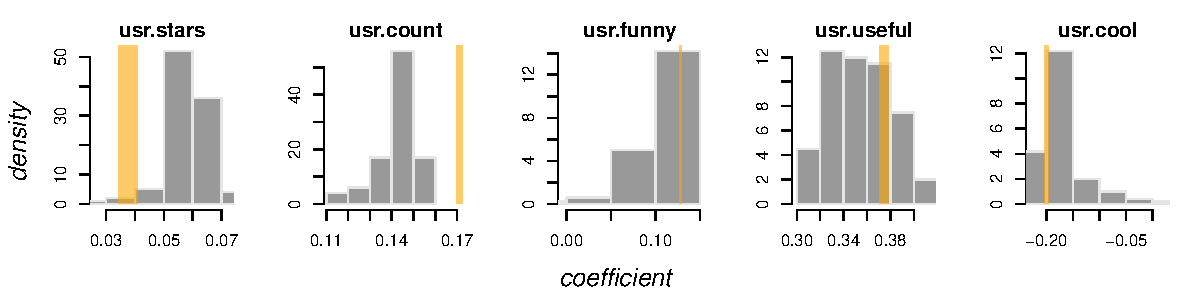
\includegraphics[width=6.35in]{../graphs/yelp_boots}
\caption{\label{boots} {\it Yelp.}  Inference for user effects.  The histograms show $100$ bootstrapped coefficient estimates in a model that regresses $y_i$ on attributes $\bm{u}_i$ and on the MNIR projections for both vote data ($\bm{z}^v_i$) {\it and} for 
the user variables of interest (the \cd{user.*} columns of $\bm{z}^u_i$).  The orange regions mark 95\% confidence intervals ($\pm 2\mr{se}$) for the corresponding MLE coefficients in regression of $y_i$ 
on $\bm{u}_i$ alone.}
\end{figure}

\section{Discussion}
\label{END}

The distribution of MNIR has opened the opportunity for it to be applied on a new  scale, one that is limited only by the number of machines you are able procure.  This includes applications where our attribute sets include a large number of fixed or even, in iterative block relaxation algorithms, latent random effects.  

This advance is important for our applied work.  The collapsing of \cite{taddy_multinomial_2013} is useful in pure prediction problems, but today we more often find ourselves addressing inference questions  of the type in Section \ref{INFER}.  High dimensional attribute sets are essential for such problems because the MNIR model needs to believable. This is in contrast to pure prediction problems where, as outlined in \cite{taddy_rejoinder:_2013}, one can model IR misspecification during forward regression.  Moreover, in social science collaboration and in business settings we've found it very valuable to have available a large set of text projections that one can call upon as required.  

Finally, the message of this paper has been that Poissson regression (or, via
Appendix \ref{WLS}, even weighted least squares) enables fast and distributed
algorithms for approximating multinomial distributions.  It has been pointed
out to us that, in unstructured data analysis, a Poisson seems little more
arbitrary than a multinomial model.  Equation (\ref{embed}) clarifies
this issue:  the only additional assumption one makes by working with
independent Poissons is that the aggregate total, $m_i$, is Poisson.  We've
attempted to mitigate the influence of this assumption, but that is
unnecessary if you consider the Poisson a fine model in and of itself.


\sgl\small
\bibliographystyle{chicago}
\bibliography{dmr}

\appendix
\dbl
\normalsize

\section{Weighted least squares approximation}
\label{WLS}

Weighted least squares (WLS) minimization works well with Big data.  Because the effect of a coefficient change on the likelihood gradient depends only on the covariances between covariates, one can pre-calculate $\bm{X}'\bm{X}$, where $\bm{X}$ is your matrix of covariates, and never again bother summing over the $n$ observations.
Our use of an IRLS algorithm for estimating Poisson log regressions (Section \ref{GL}) begs the question: can we fix the weights? 

The Poisson regression model for $c_i$ has intensities $e^{\eta_{i}}$, suppressing response-category subscript $j$. Then
 $\bs{\eta} = [\eta_{1} \ldots \eta_{n}]$ is our estimation target,
with likelihood Hessian matrix $\bm{H} = \mr{diag}(e^{\eta_{i}})$.
Expand a second order Taylor series around the saturated model $\hat\eta_{i}
= \log(c_{i})$ (so the gradient disappears) to get the approximate negative
log likelihood 
\begin{equation}
l(\bs{\eta}) = (\bs{\eta} - \log\bm{c})'
\mr{diag}( \bm{c} )(\bs{\eta} - \log\bm{c}). 
\end{equation} 
Writing $\bs{\eta}$
out in terms of our fixed-effects regression model yields the approximate
Poisson negative log LHD objective $\sum_i c_{i}(\alpha +
\bm{v}_i'\bs{\varphi} - \log(c_{i}/m_i))^2$, a sum of squares with weights $c_{i}$ ($=c_{ij}$ for each response $j$). This formula will not work in application due to all of the zero values $c_i$, but we can add a small buffer term $\zeta > 0$ to get the {\it WLS Poisson approximation}
\begin{equation}\label{wls}
l(\alpha, \bs{\varphi}) = \sum_i \omega_i
\left[\alpha_j + \bm{v}_i'\bs{\varphi} - \log(\omega_i/m_i)\right]^2, ~~\text{where}~~\omega_i = c_i + \zeta.
\end{equation}
Effect of $\zeta$ is clearest around $c_i = 0$: as the buffer decreases, the weights $\omega_i$ get smaller while the distance from `response' $\log(\omega_i/m_i)$ to that for $c_i=1$, $\log( [1+\zeta]/m_i )$, gets larger.

\begin{figure}
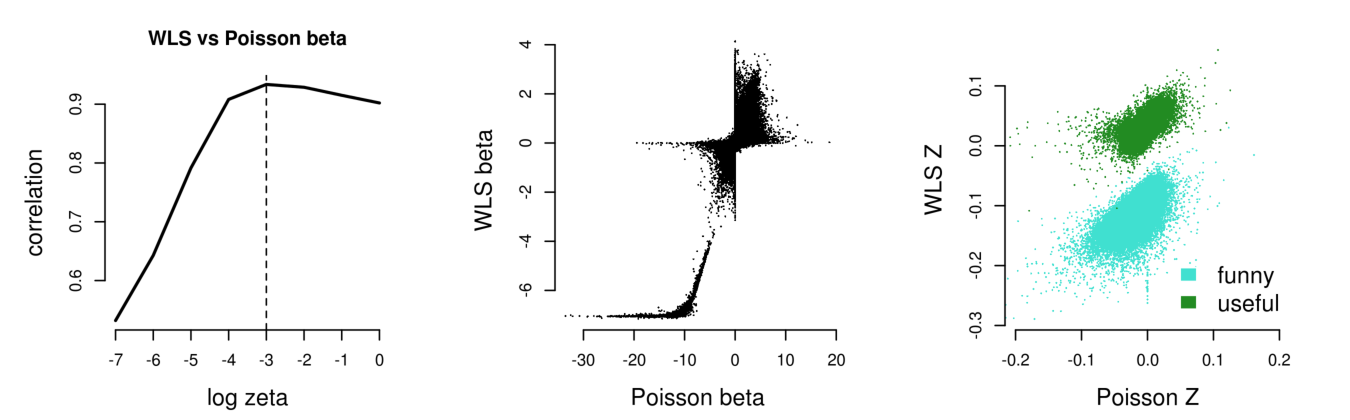
\includegraphics[width=6.5in]{../graphs/wlscompare}
\caption{\label{wlspic} {\it Yelp.} Weighted least squares approximation.  The left plot shows correlation between  Poisson coefficient estimates and the WLS values, as a function of buffer $\zeta$. At marked $\zeta=e^{-3}\approx 1/20$, the center graph plots the estimated values under each method against each other and the right panel shows projection onto two vote categories (useful and cool overlap very closely, so we've left cool unplotted).}
\end{figure}


The left panel of Figure \ref{wlspic} shows correlation  between  MNIR
$\bs{\hat\Phi}$ estimates obtained, after AIC model selection,  from a Poisson
likelihood and from our WLS approximation.  The fits are impressively close,
especially given that this involves  selection after estimation, with a
maximum correlation of $0.94$ at $\zeta=0.05$.  The center panel shows that
there are systematic discrepancies:  WLS estimates are attenuated,
and some big negative $\hat\varphi_{ij}$ estimates from the Poisson fit are
thresholded around $-7$ in WLS.  However, the right plot shows that this does
not necessarily carry into the implied SR projections. Of primary importance,
OOS predictability for MNIR is practically unchanged.  Cross validation with
$\zeta=0.05$ for the Yelp example from Section \ref{YELP}, in the same
experiment of Figure \ref{yelp_cv}, yields OOS $R^2$  values of
0.454 for a linear forward model and 0.520 for a random forest -- only 0.001
lower than for the exact likelihood.

\end{document}
